\documentclass{article}

\usepackage{AcademicReport}

% enable Chinese
% \usepackage[UTF8]{ctex}


% setting for levels
\usepackage{hyperref}
\setcounter{secnumdepth}{2}
\setcounter{tocdepth}{2}
\hypersetup{
    bookmarksopenlevel = 3,
    citecolor = red,
	colorlinks		=	true,
	bookmarks		=	true,
	bookmarksopen	=	true,
    % bookmarksdepth  =   2,
	pdfstartview	=	Fit,
	pdftitle		=	{Academic Report Template},
	pdfauthor		=	{Jiaxin Zhong},
}

% open book mark at arbitrary level
\usepackage[open, numbered]{bookmark}
% opt: numbered --- show numbers in the bookmark

% for some dummy text
\usepackage{lipsum}

% see https://tex.stackexchange.com/questions/226481/appendix-section-title
\usepackage[title]{appendix}


\title{\textbf{Experimental Notes for the Underwater Acoustic Metamaterial Project}}
\author{Jiaxin Zhong}
\date{\today}

% \usepackage{mlmodern}


\begin{document}
\maketitle
% enable Page 1 of xx at the first page
\thispagestyle{firststyle}

\section{Introduction}
Experiments were conducted to validate the enhanced transmission through an underwater acoustic metamaterial (AMM).

\subsection{General settings}

\begin{table}[!htb]
    \centering
    \caption{Comparison of retrieved parameters.}
    \begin{tabular}{llll}
        \toprule
        Name & Symbol & Value & Comments 
         \\
        \midrule
        Emitter radius
             &  -- & 1 inch & -- 
             \\
             Metamaterial dimensions
             & --
             & $\SI{29}{mm} \times \SI{29}{mm}$
             & --
             \\
            Center frequency 
                 & $f_\mathrm{c}$
                 & 445~kHz & --
             \\
             Wavelength
                 & $\lambda_\mathrm{c}$
                 & 3.3~mm & --
            \\
             Critical distance
                 & $D_\mathrm{c} = a^2/\lambda_\mathrm{c}$
             & 68.2~mm
             & --
            \\
        \bottomrule
    \end{tabular}
    \label{tab:param}
\end{table}

\section{Experimental logs}
Equipment settings are:
\begin{itemize}
    \item Oscilloscope
        \begin{itemize}
            \item y division 1~V
            \item x division 5~MHz
        \end{itemize}
    \item Function generator
        \begin{itemize}
            \item Vpp is 5~V
            \item Burst mode, 1~ms period, 5~cycles
        \end{itemize}
\end{itemize}

\subsection{Exp230223B}
\label{sec:exp230223B}
\begin{itemize}
    \item DDate: Feb 23, 2023
    \item Measurement of the transmitted sound field without AMM
\end{itemize}

\subsection{Exp230227B}
\label{sec:exp230227B}

\subsubsection{Specific settings}
\begin{itemize}
    \item Date: Feb 27, 2023
    \item Measurement of the transmitted sound field with AMM
\end{itemize}

\subsection{Exp230228A}
\label{sec:exp230228A}
\begin{itemize}
    \item AMM
    \item Transmistted sound field over the plane $y=\SI{46}{mm}$.
\end{itemize}

\subsection{Exp230228F}
\label{sec:exp230228F}
\begin{itemize}
    \item AMM
    \item Transmistted sound field over the plane $y=\SI{45.75}{mm}$.
\end{itemize}

\subsection{Exp230301D}
\label{sec:exp230301D}
\begin{itemize}
    \item AMM
    \item Transmistted sound field over the plane $y=\SI{45.5}{mm}$.
\end{itemize}

\subsection{Exp230302A}
\label{sec:Exp230302A}
\begin{itemize}
    \item Without AMM
    \item Transmistted sound field over the plane $y=\SI{46}{mm}$.
\end{itemize}

\subsection{Exp230302B}
\label{sec:Exp230302B}
\begin{itemize}
    \item Without AMM
    \item Transmistted sound field over the plane $y=\SI{45.75}{mm}$.
\end{itemize}

\subsection{Exp230302G}
\label{sec:Exp230302G}
\begin{itemize}
    \item Without AMM
    \item Transmistted sound field over the plane $y=\SI{45.5}{mm}$.
\end{itemize}

\subsection{Exp230303A}
\label{sec:Exp230303A}
\begin{itemize}
    \item With plate
    \item Horizontal plane
\end{itemize}

\subsection{Exp230306A}
\label{sec:Exp230306A}
\begin{itemize}
    \item With plate
    \item Vertifcal plane at $y=\SI{46}{mm}$
\end{itemize}

\subsection{Exp230307A}
\label{sec:Exp230307A}
\begin{itemize}
    \item With plate
    \item Vertifcal plane at $y=\SI{46}{mm}$
\end{itemize}

\subsection{Exp230307B}
\label{sec:Exp230307B}
\begin{itemize}
    \item With plate
    \item Vertifcal plane at $y=\SI{45.75}{mm}$
\end{itemize}


\section{Results and discussions}
Figure~\ref{fig:39:f020390} shows the results of someting.
\begin{figure}[!htb]
    \centering
    \begin{subfigure}{0.32\textwidth}
        \centering
        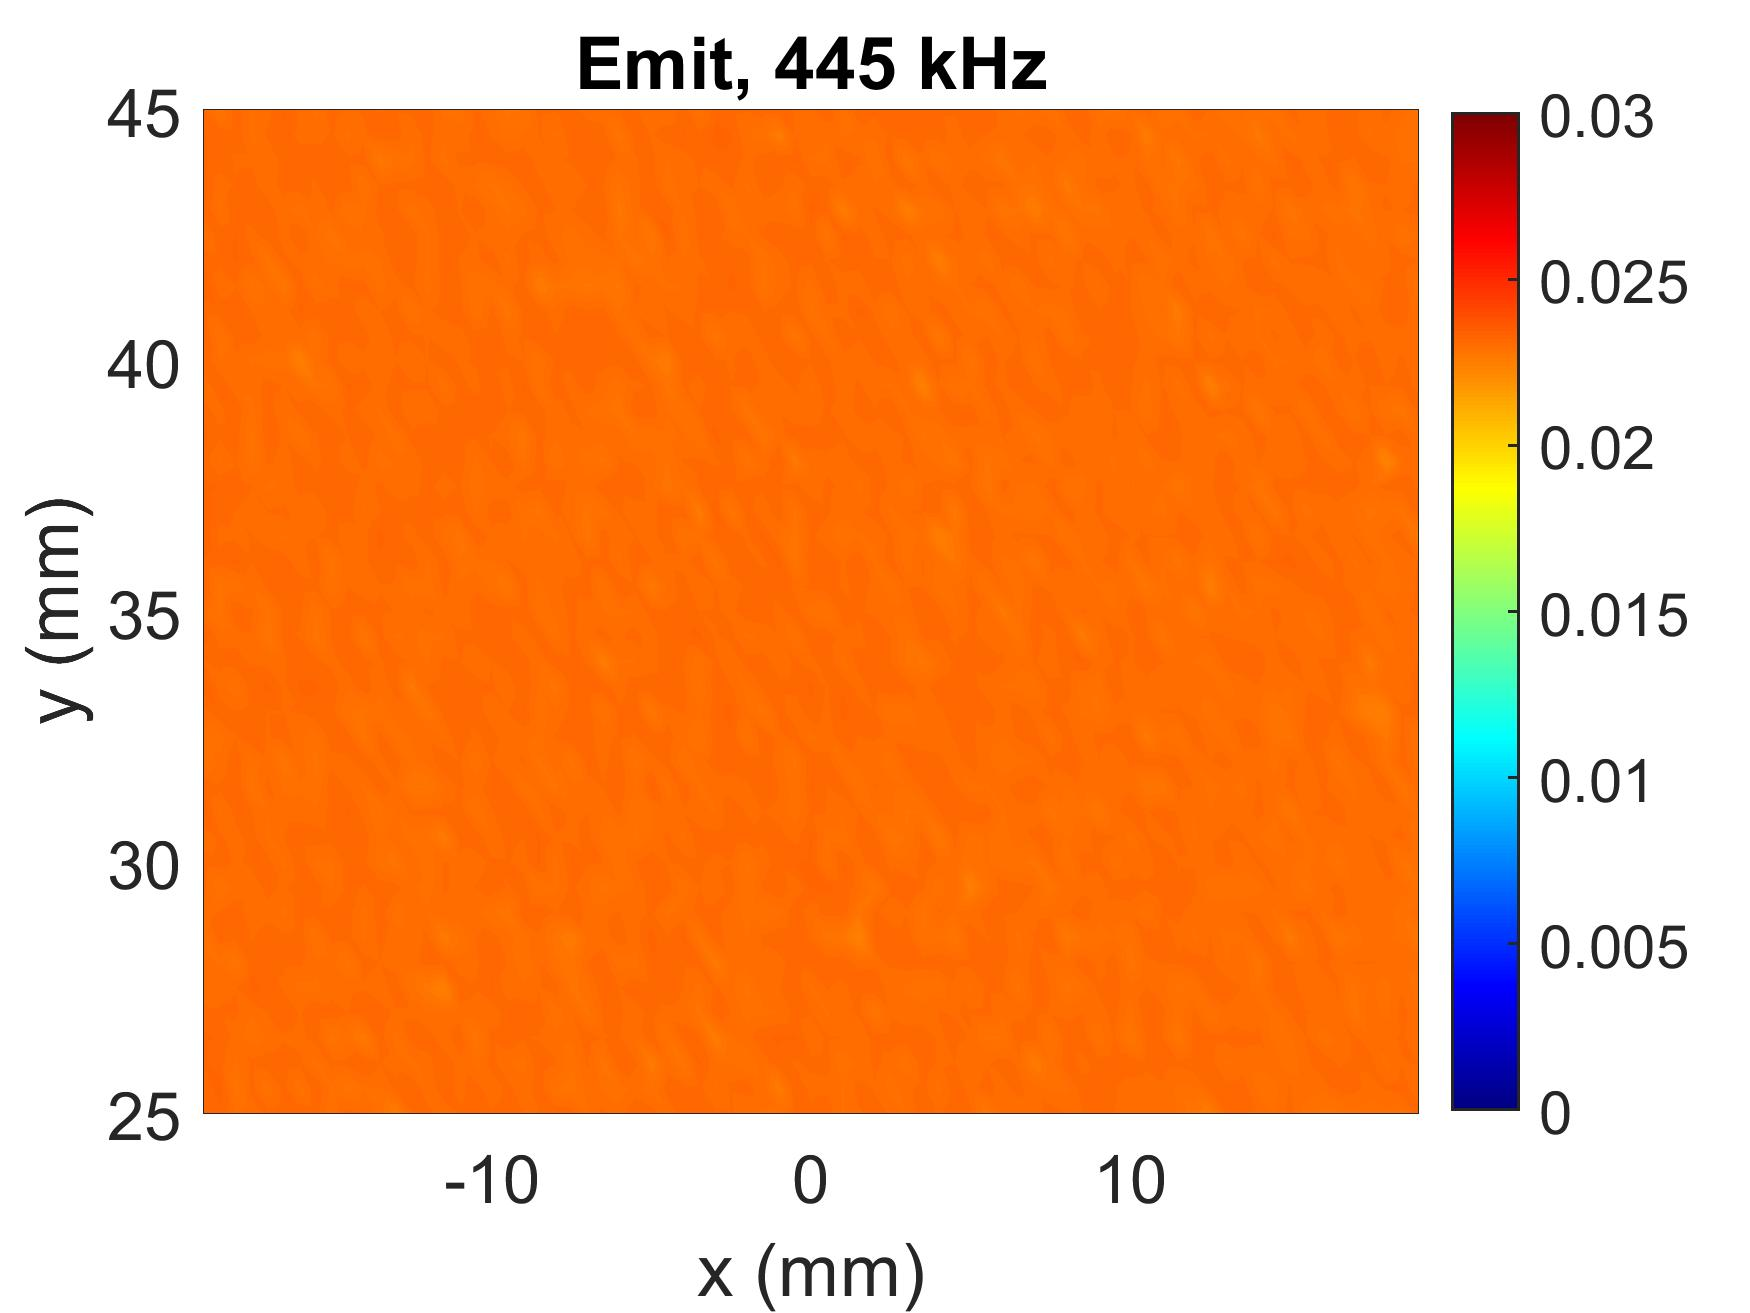
\includegraphics[width = \textwidth]{../../matlab/exp/fig/AnalyzeData_230227D_Exp230223B_EmitPrs}
        \caption{}
    \end{subfigure}
    \begin{subfigure}{0.32\textwidth}
        \centering
        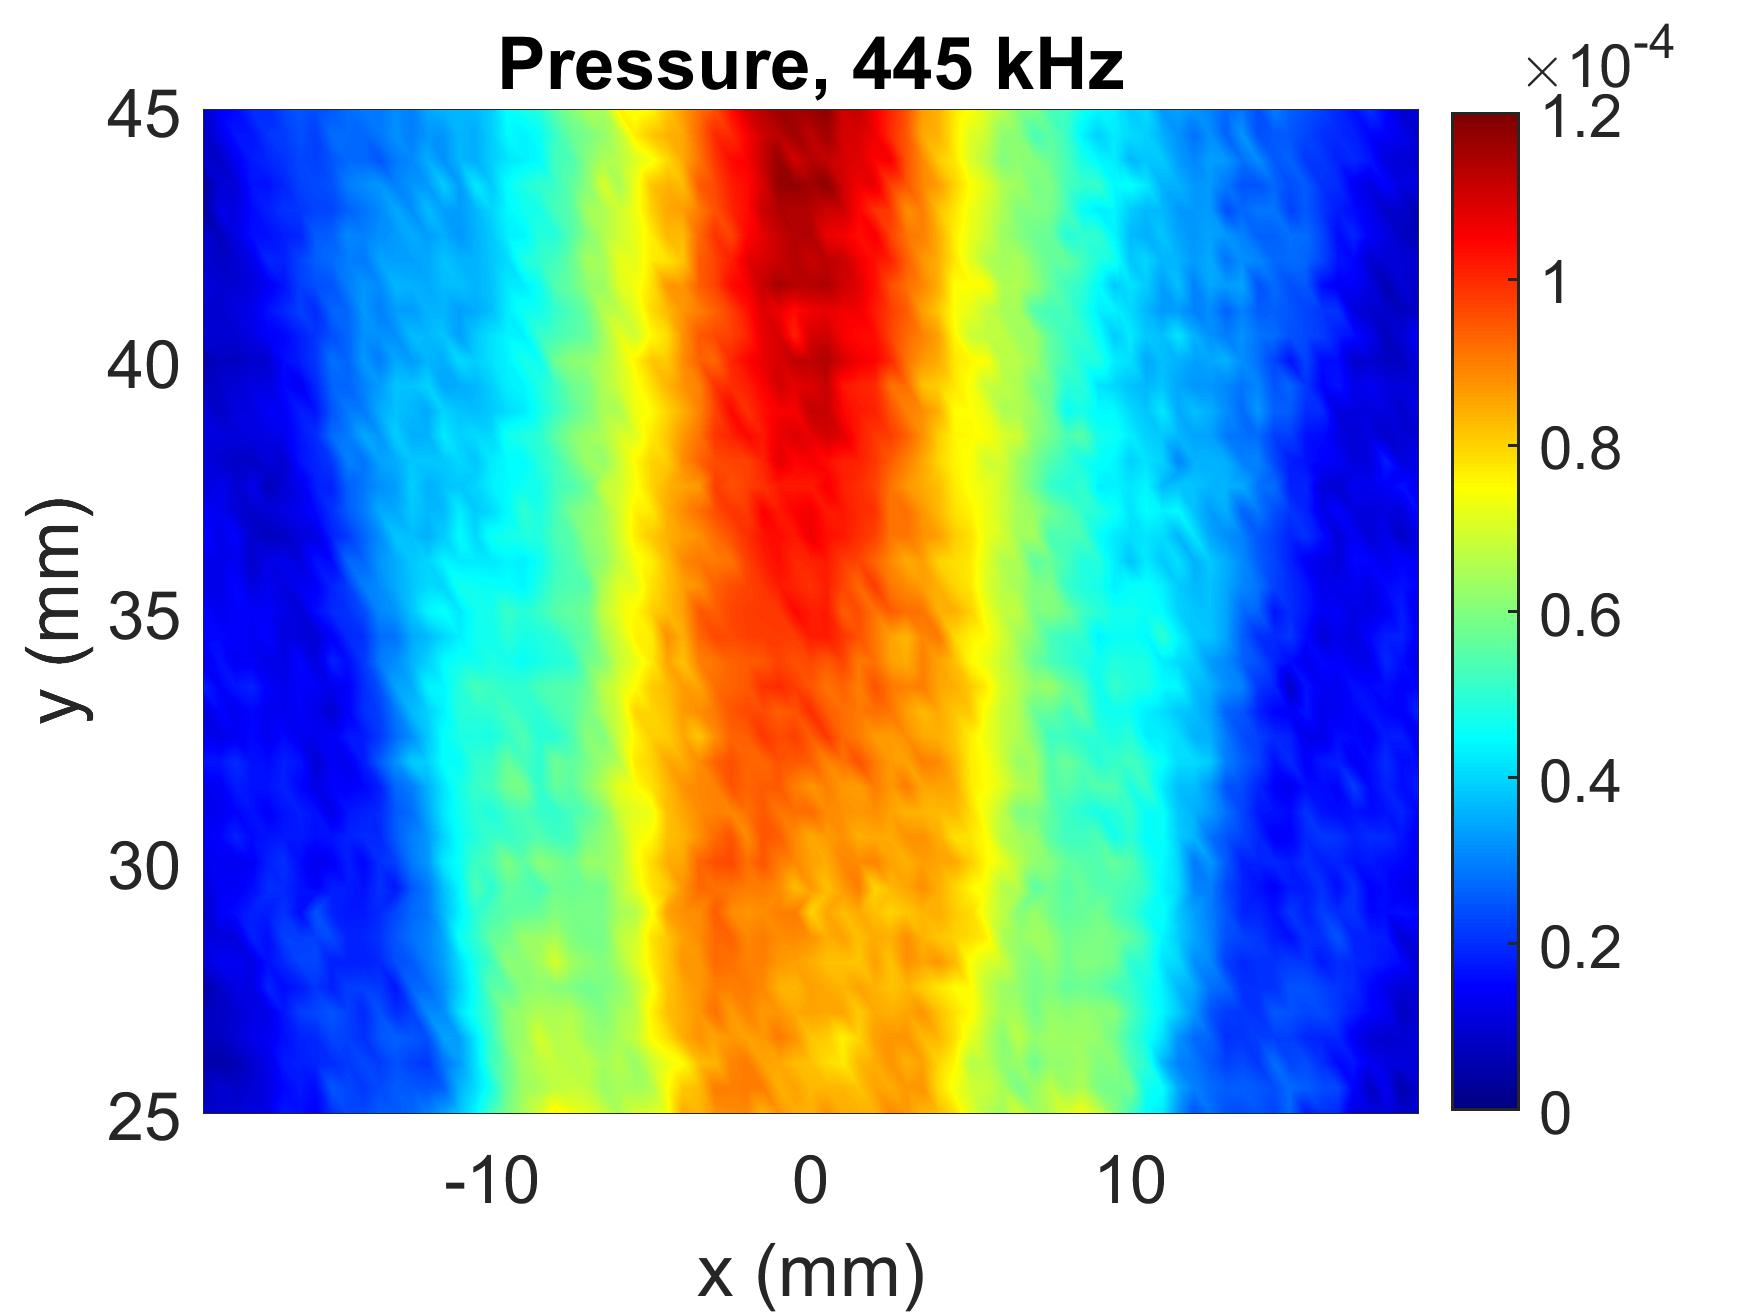
\includegraphics[width = \textwidth]{../../matlab/exp/fig/AnalyzeData_230227D_Exp230223B_RecPrs.jpg}
        \caption{}
    \end{subfigure}
    \begin{subfigure}{0.32\textwidth}
        \centering
        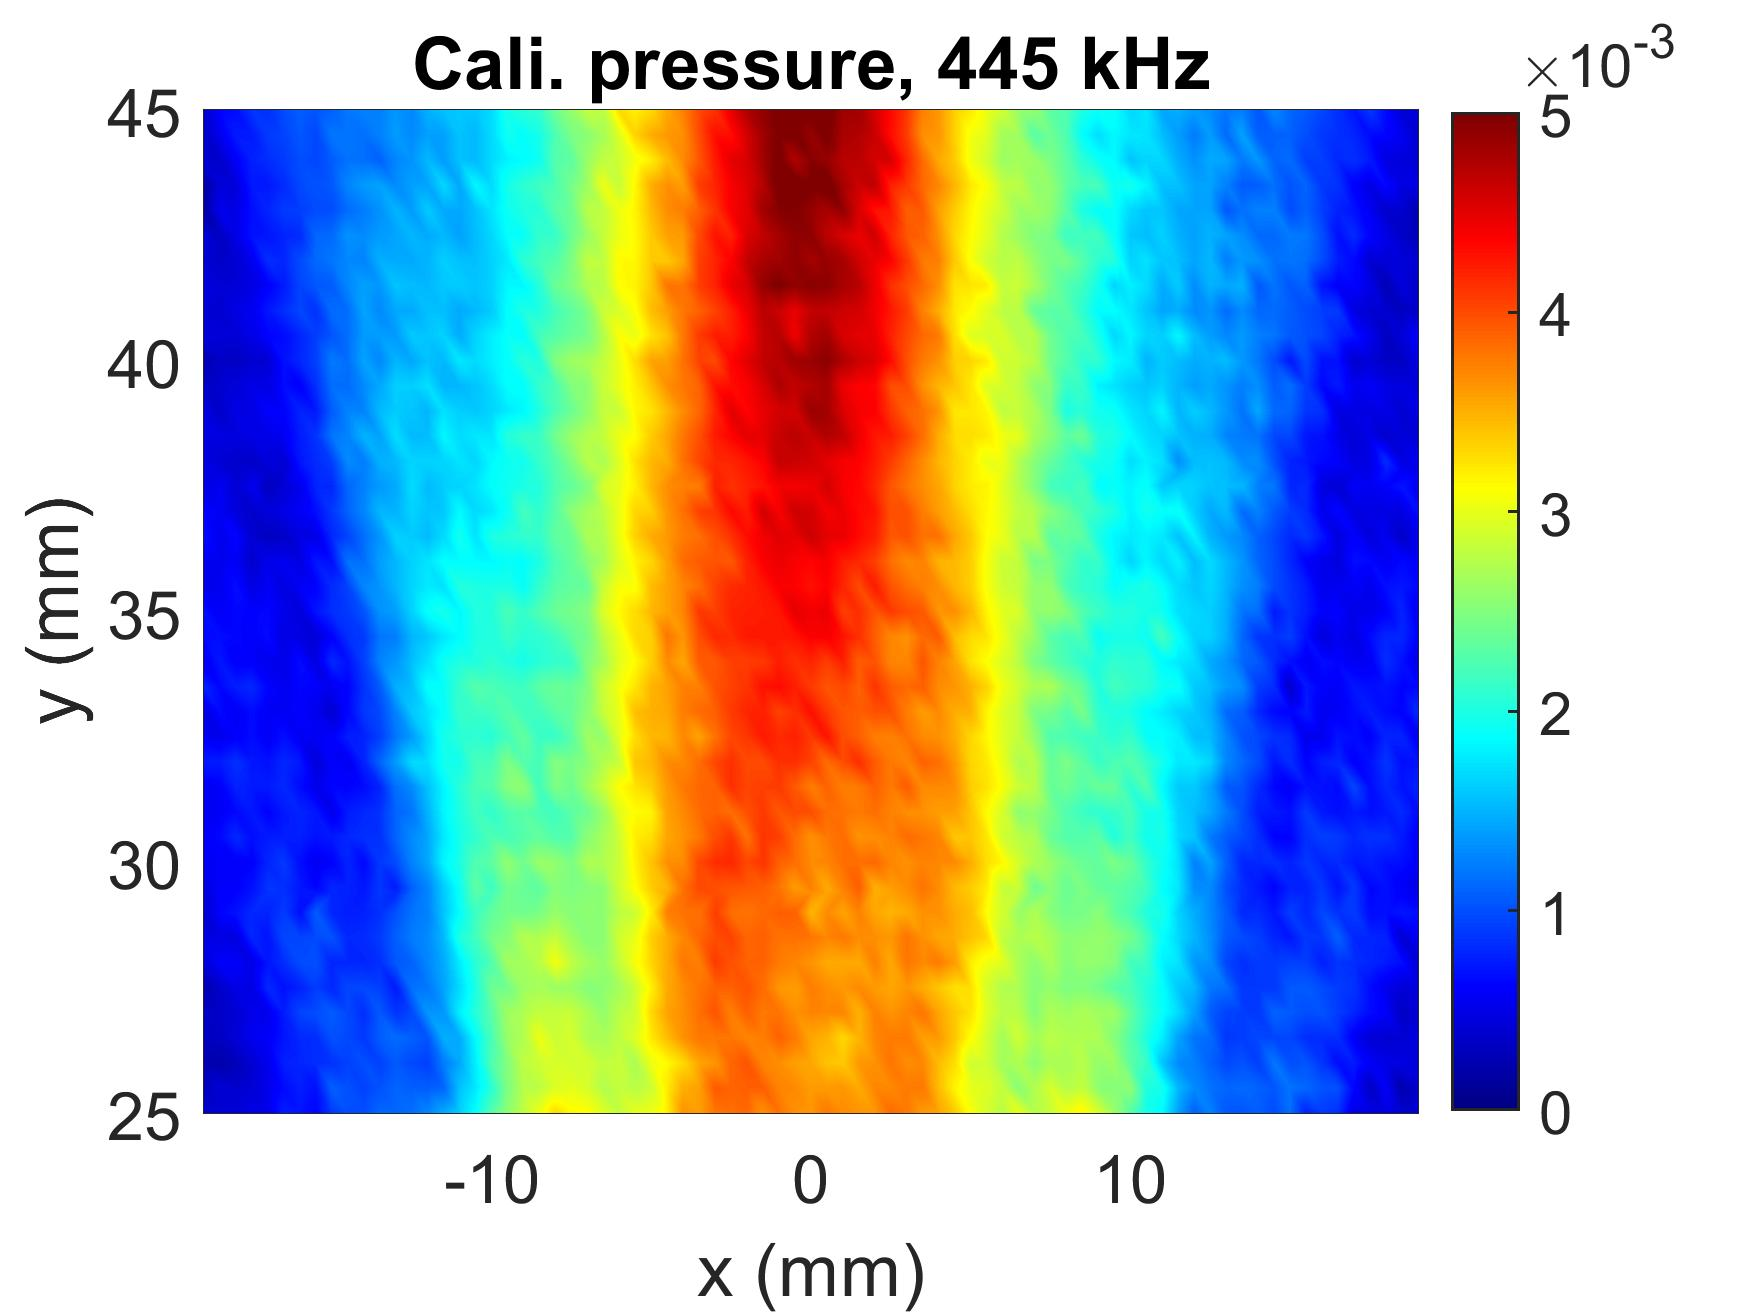
\includegraphics[width = \textwidth]{../../matlab/exp/fig/AnalyzeData_230227D_Exp230223B_CaliRecPrs.jpg}
        \caption{}
    \end{subfigure}
    \\
    \begin{subfigure}{0.32\textwidth}
        \centering
        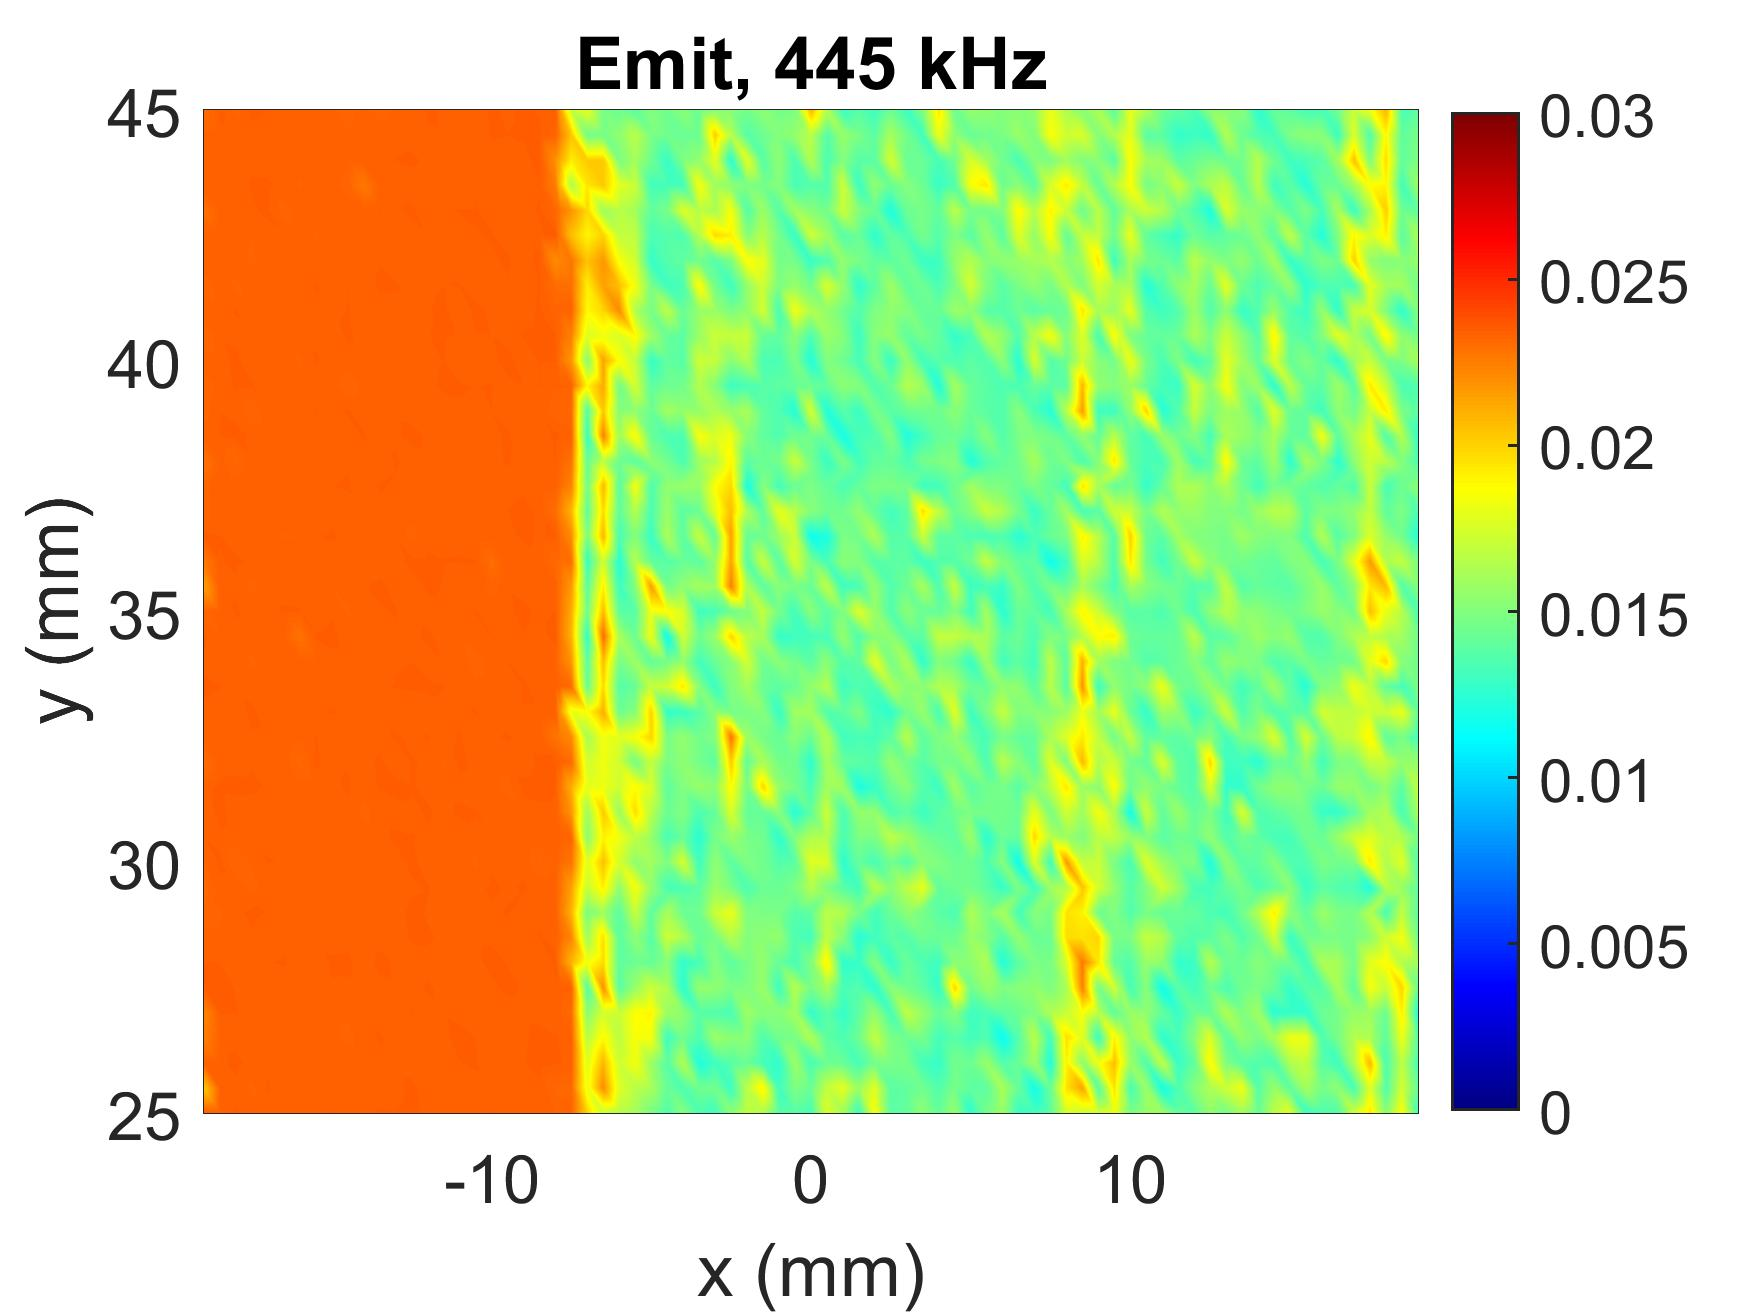
\includegraphics[width = \textwidth]{../../matlab/exp/fig/AnalyzeData_230227D_Exp230227B_EmitPrs}
        \caption{}
    \end{subfigure}
    \begin{subfigure}{0.32\textwidth}
        \centering
        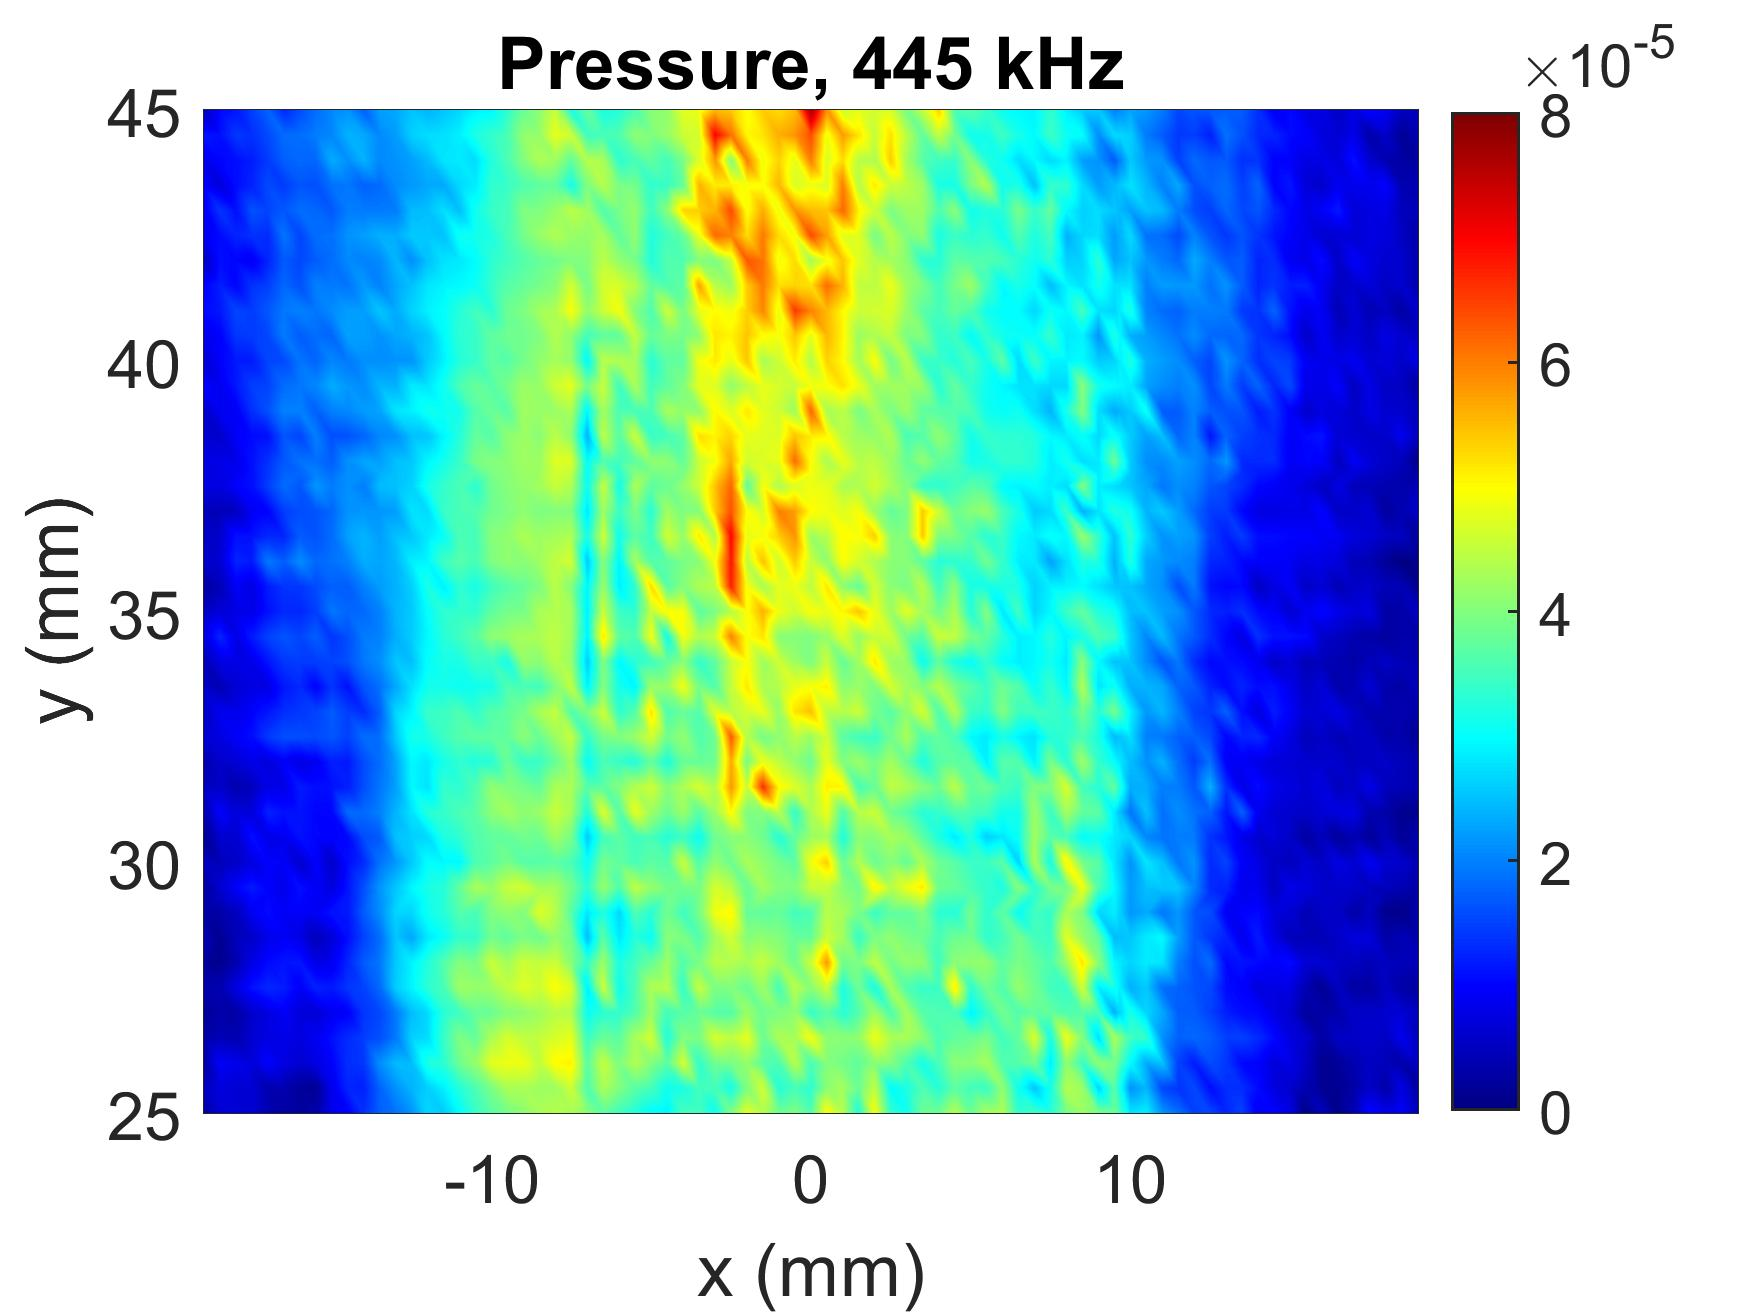
\includegraphics[width = \textwidth]{../../matlab/exp/fig/AnalyzeData_230227D_Exp230227B_RecPrs.jpg}
        \caption{}
    \end{subfigure}
    \begin{subfigure}{0.32\textwidth}
        \centering
        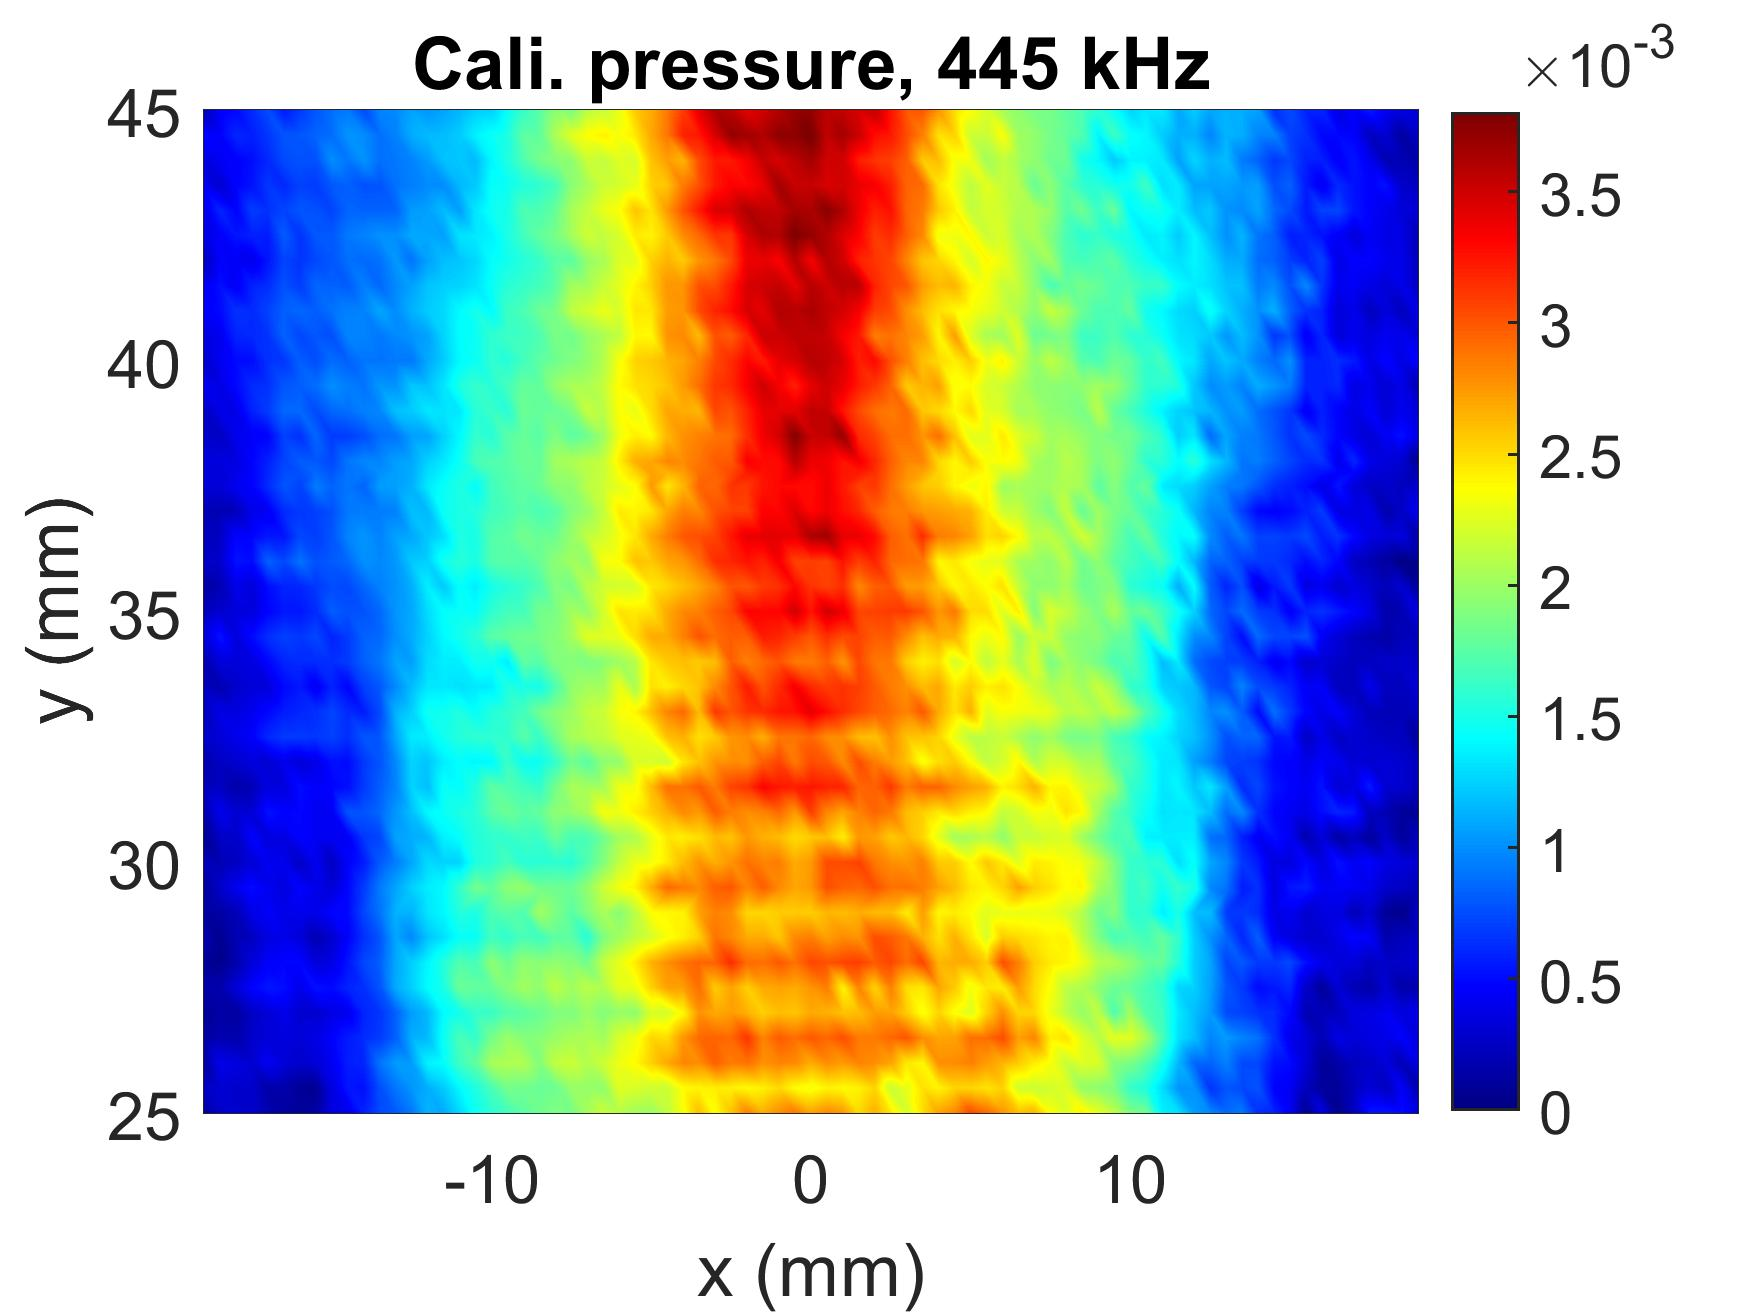
\includegraphics[width = \textwidth]{../../matlab/exp/fig/AnalyzeData_230227D_Exp230227B_CaliRecPrs.jpg}
        \caption{}
    \end{subfigure}
    \caption{2D experimental results at 445~kHz.
        Top row, without AMM (see Sec.~\ref{sec:exp230223B}); bottom row, with AMM (see Sec.~\ref{sec:exp230227B}).
        Left column, emitting signal which was fed into the source; 
        middle column, signal received by the hydrophone;
        right column, calibrated signal of the middle column.
    To calibrate, the values in the middle column are divided by those in the left column.
    }
    \label{fig:39:f020390}
\end{figure}

\begin{figure}[!htb]
    \centering
    \begin{subfigure}{0.45\textwidth}
        \centering
        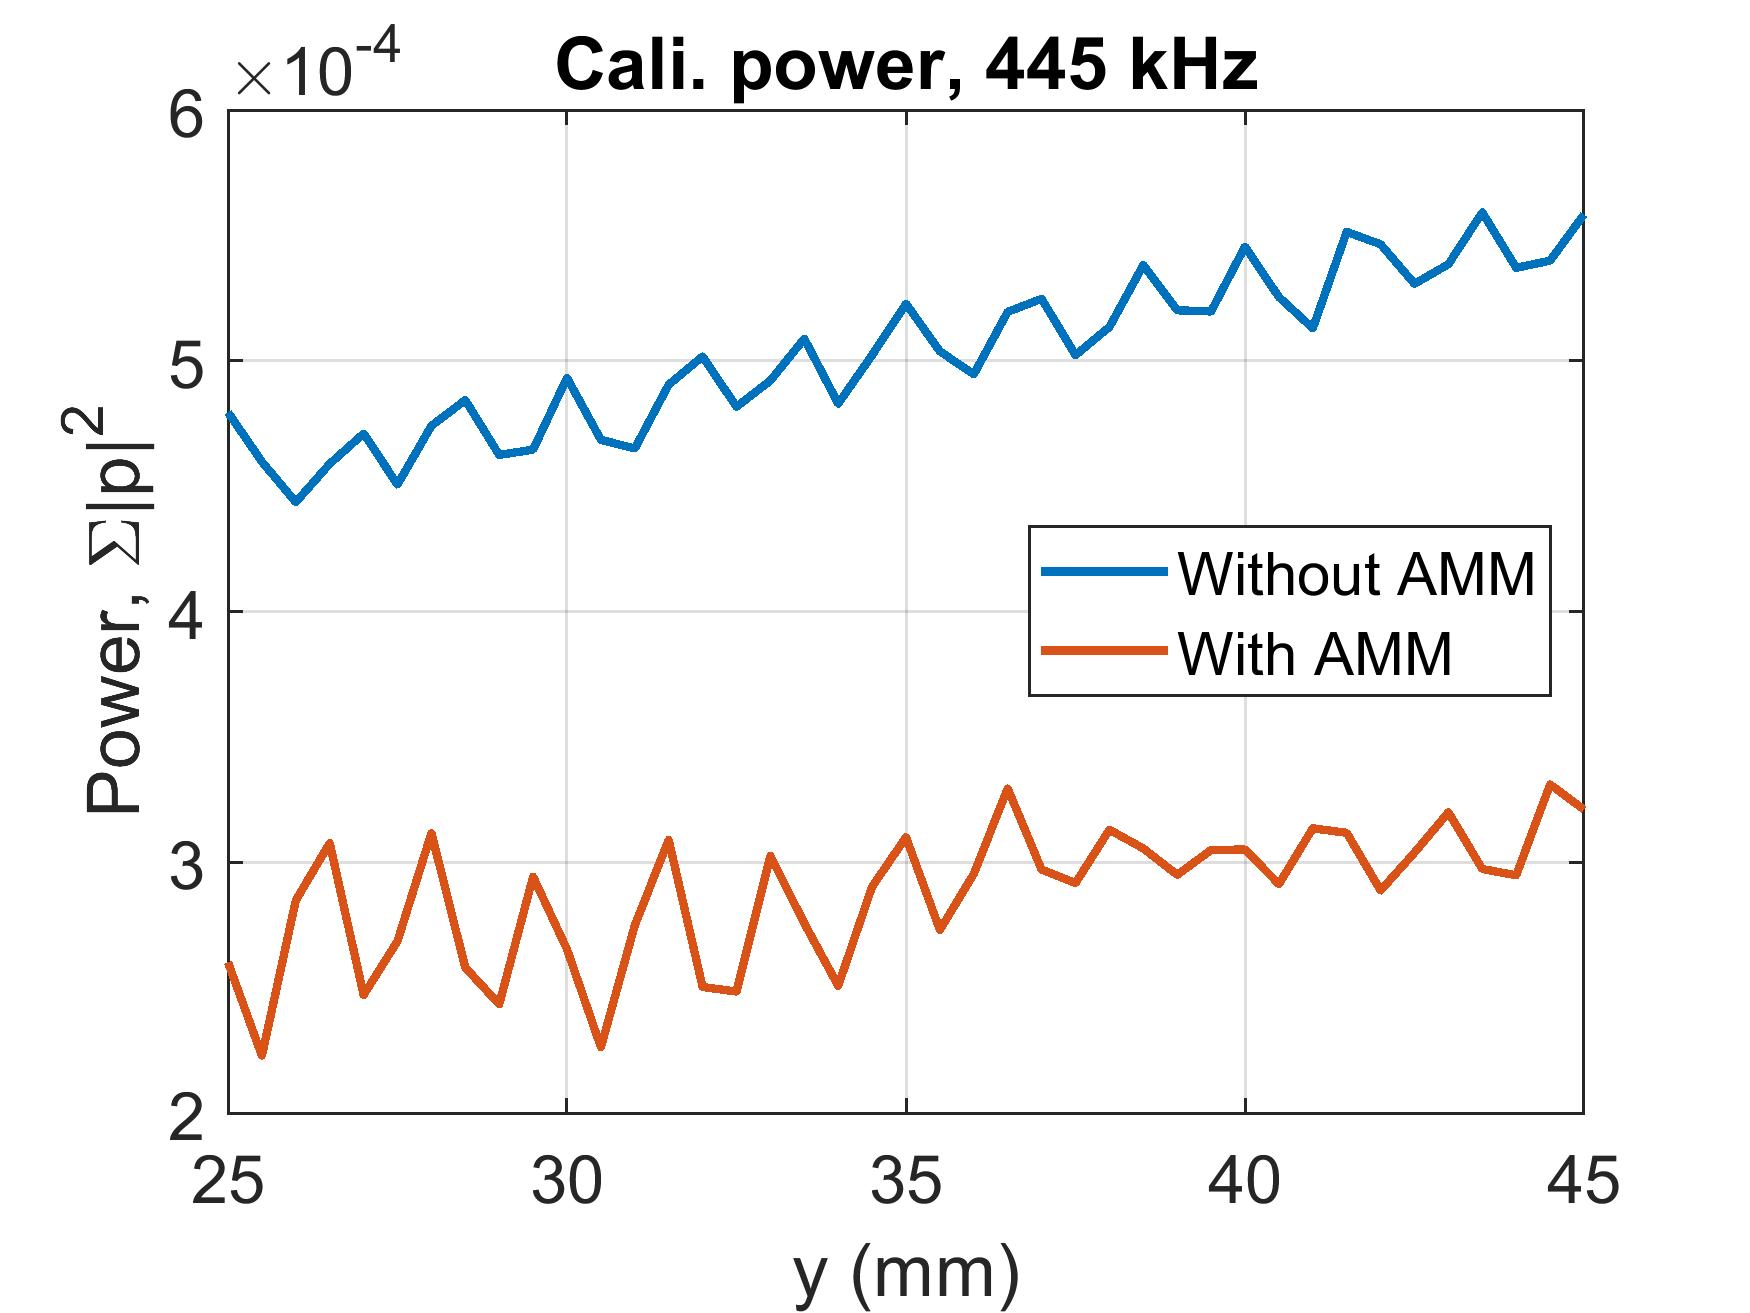
\includegraphics[width = \textwidth]{../../matlab/exp/fig/AnalyzeData_230227D_Exp230223B_Exp230227B_CaliPow}
        \caption{}
    \end{subfigure}
    \begin{subfigure}{0.45\textwidth}
        \centering
        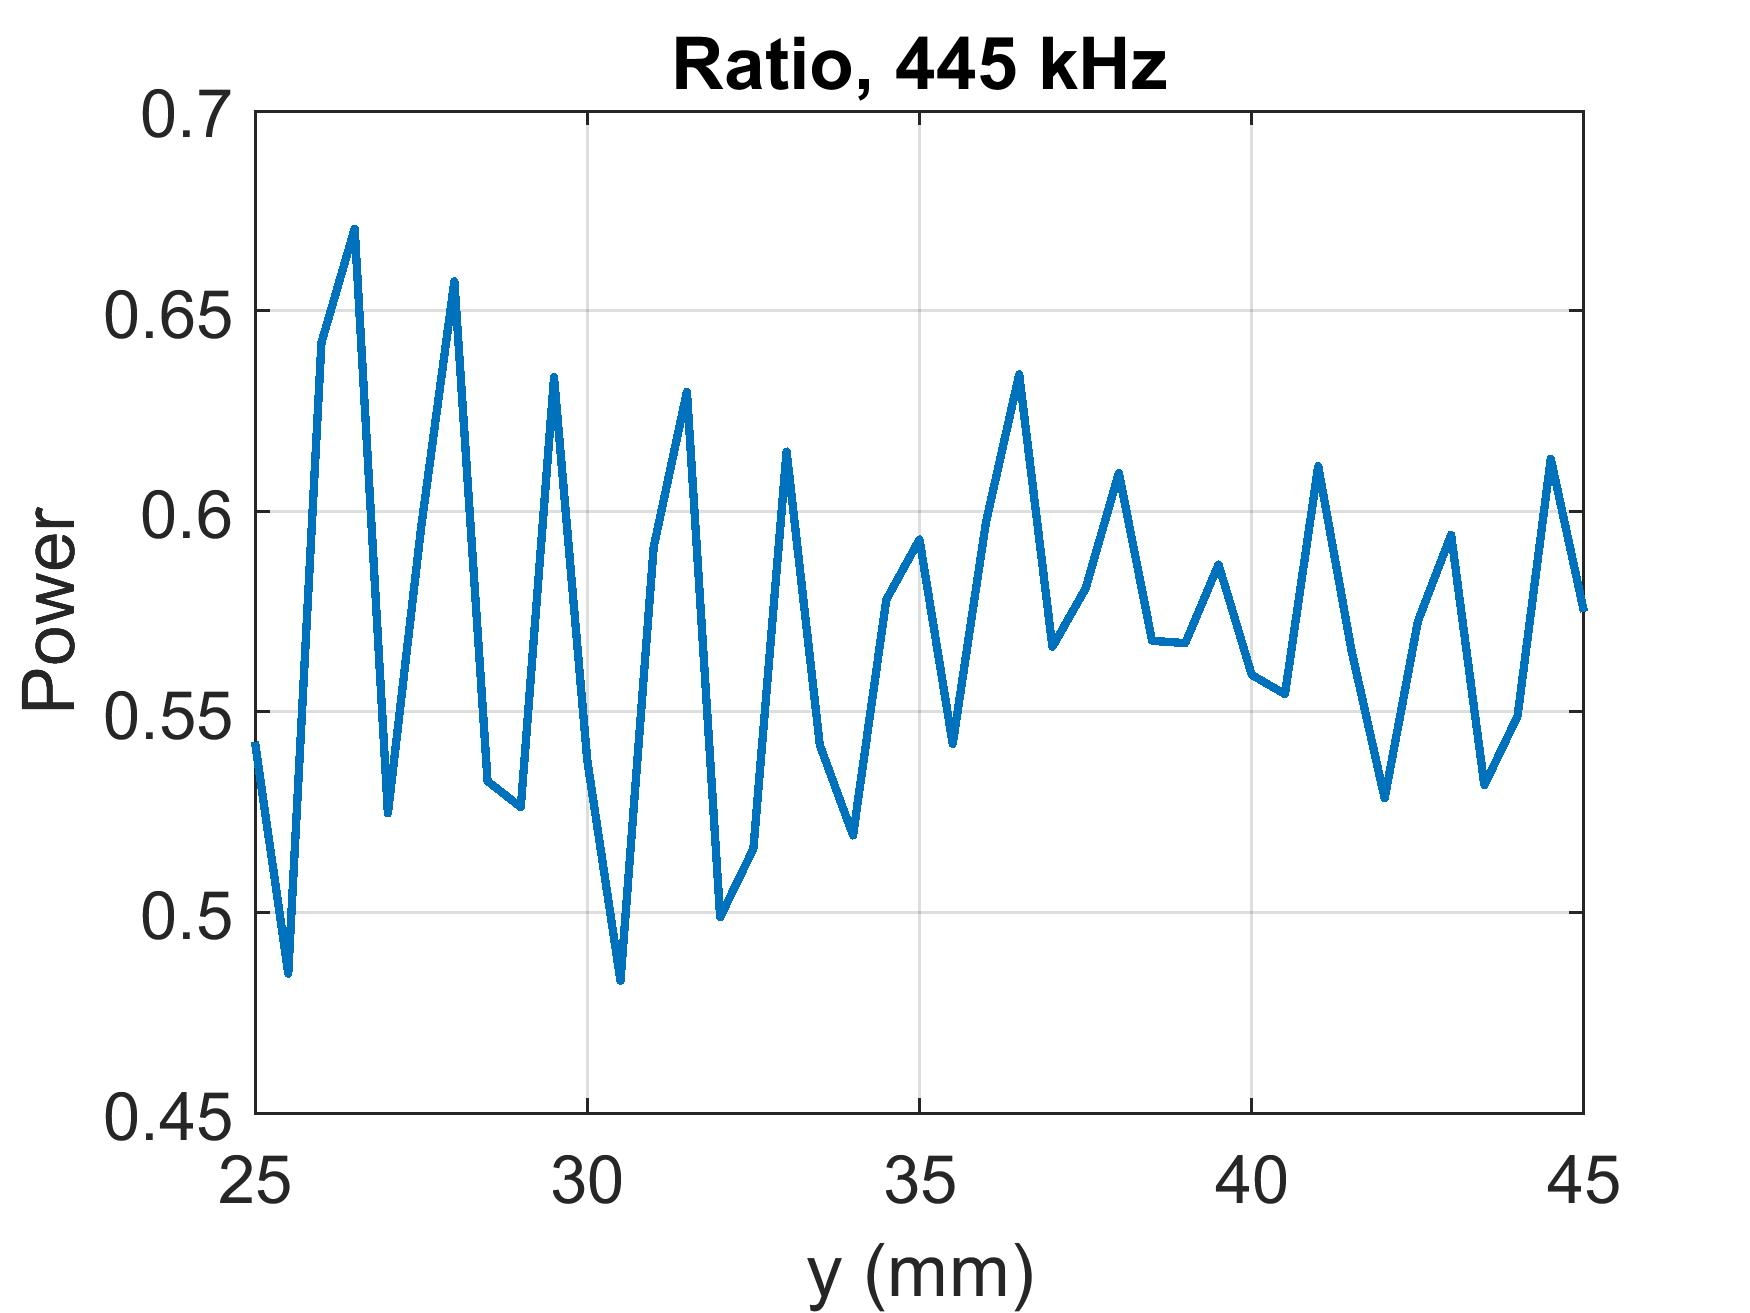
\includegraphics[width = \textwidth]{../../matlab/exp/fig/AnalyzeData_230227D_Exp230223B_Exp230227B_CaliPowRatio}
        \caption{}
    \end{subfigure}
    \caption{(a) Calibrated acoustic power, approximated by a summation of the squared pressure along the line parallel to $x$ axis, with and without AMM. 
    (b) The ratio of the power with AMM to that without AMM.}
    \label{fig:f9e:320eui203}
\end{figure}


\begin{figure}[!htb]
    \centering
    \begin{subfigure}{0.45\textwidth}
        \centering
        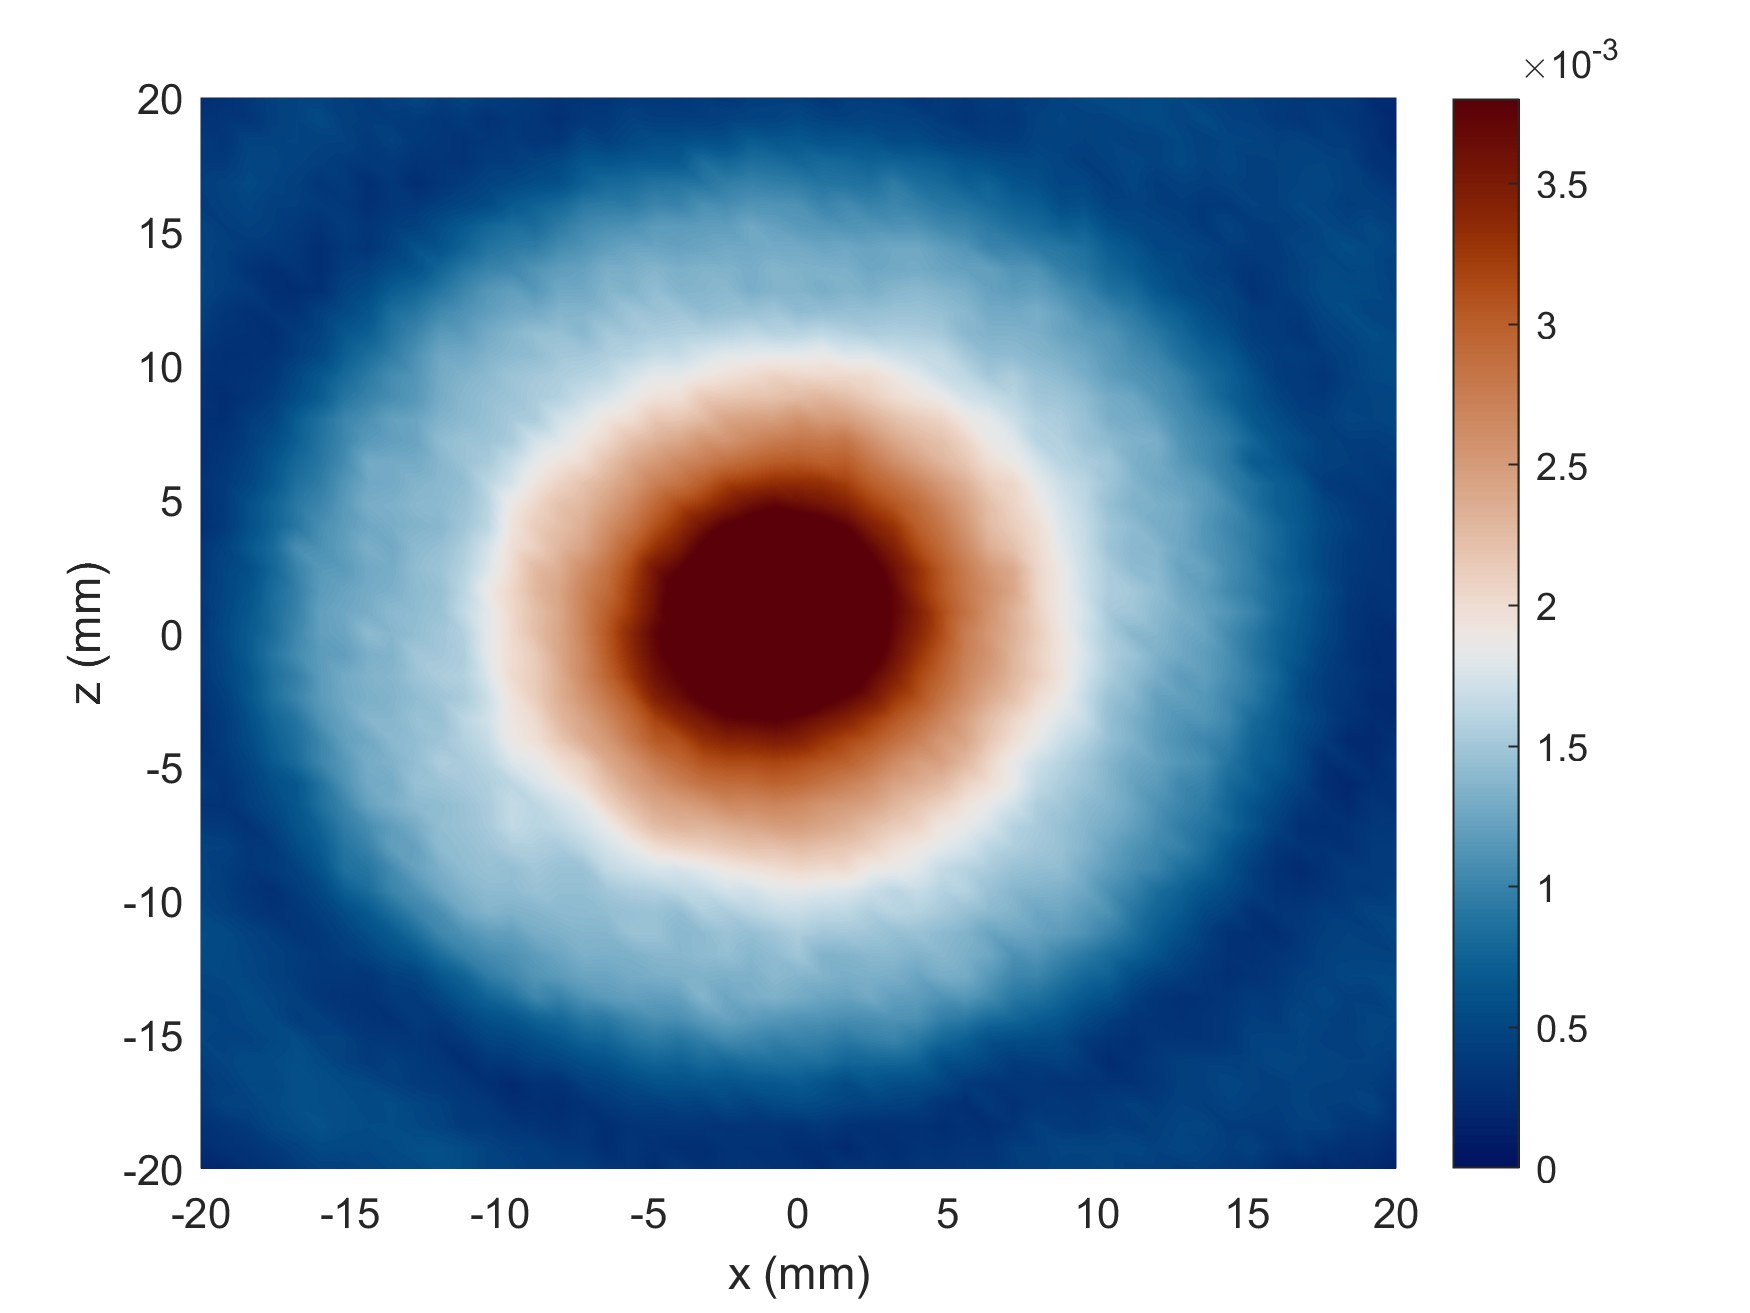
\includegraphics[width = \textwidth]{../../matlab/exp/fig/CalPowTransCoef_230302C_PrsVoid.jpg}
    \end{subfigure}
    \begin{subfigure}{0.45\textwidth}
        \centering
        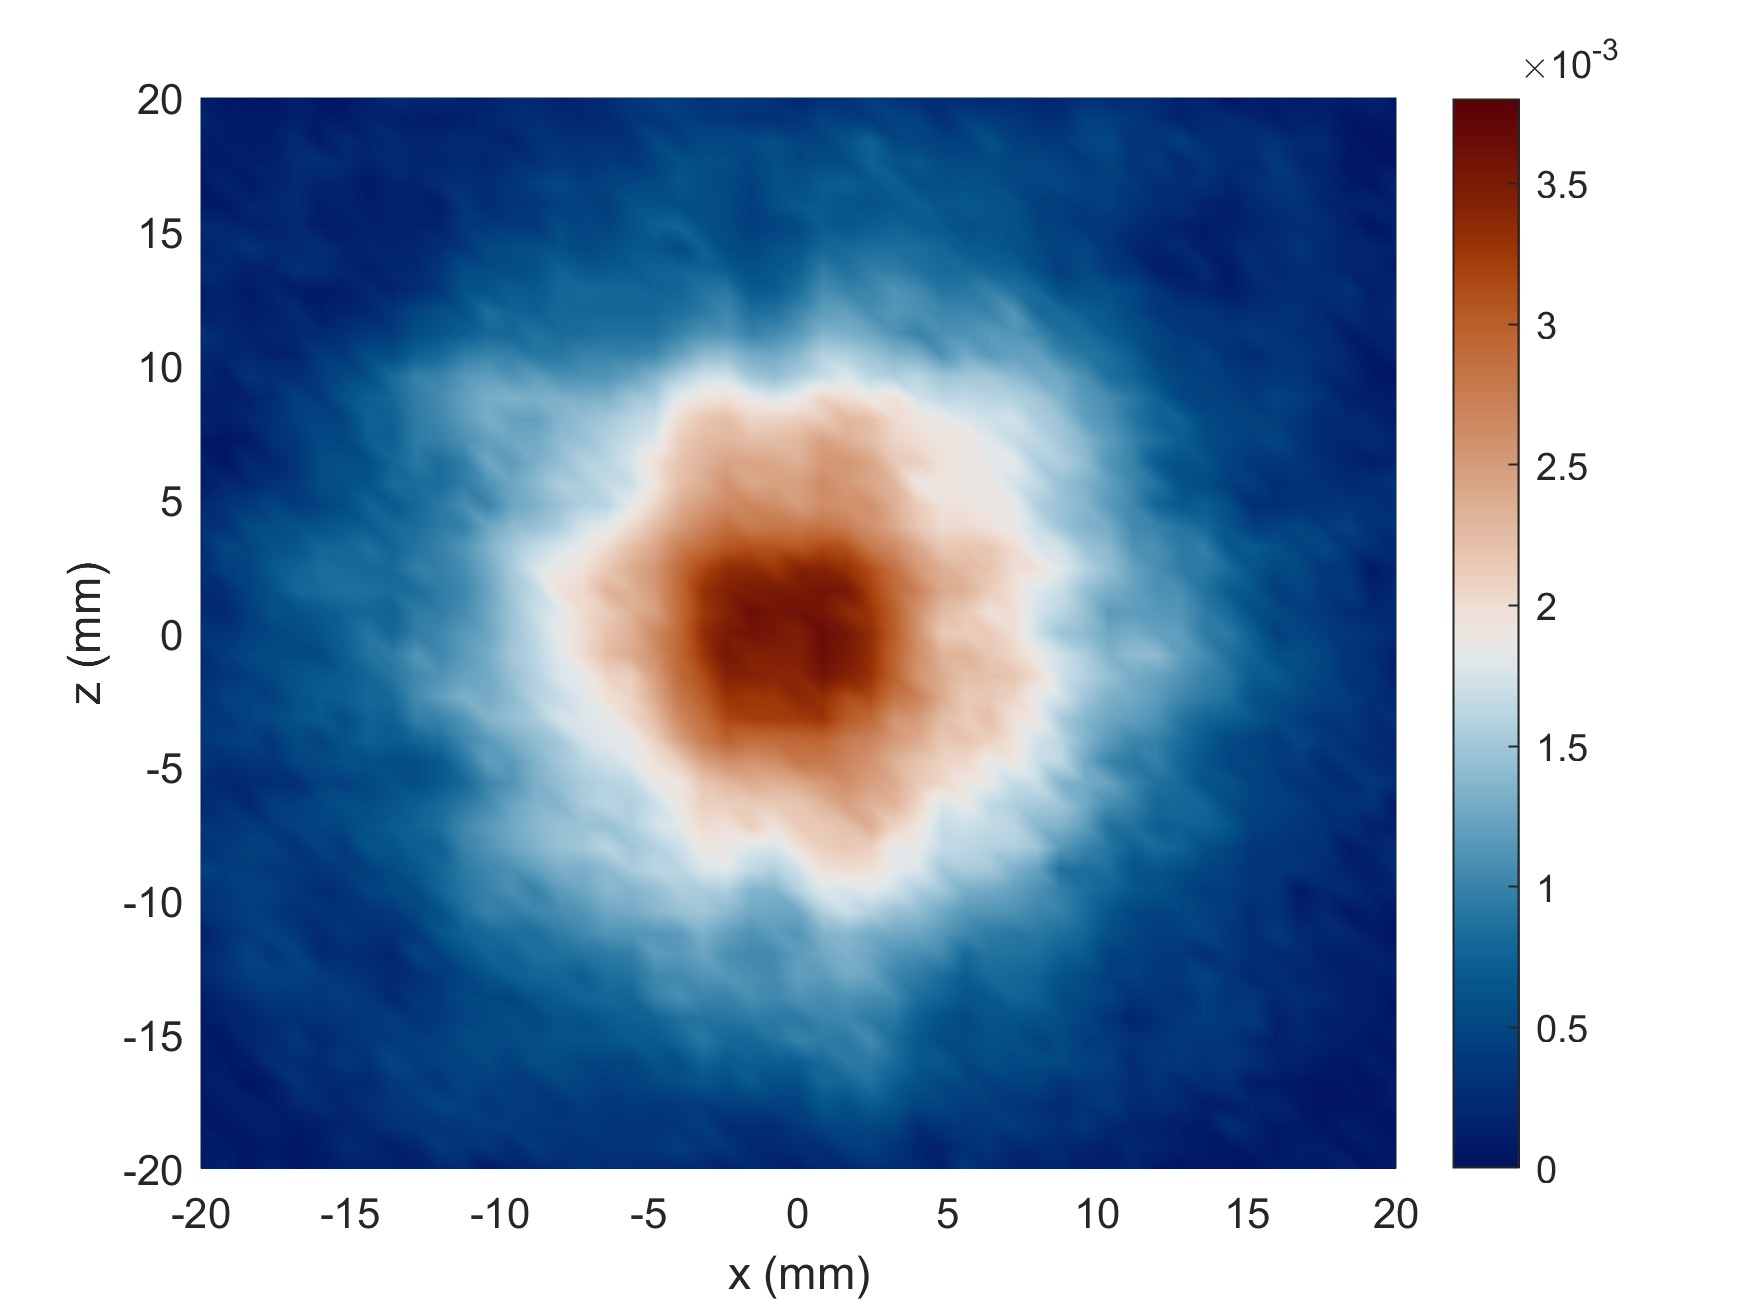
\includegraphics[width = \textwidth]{../../matlab/exp/fig/CalPowTransCoef_230302C_PrsAMM.jpg}
    \end{subfigure}
    \caption{2D pressure distribution at 445~kHz without (left) and with (right) the acoustic metamatrial (AMM).
    The region is located at 45~mm away from the transducer.}
    \label{fig:f9j:0213921j09j}
\end{figure}
\begin{figure}[!htb]
    \centering
    \begin{subfigure}{0.32\textwidth}
        \centering
        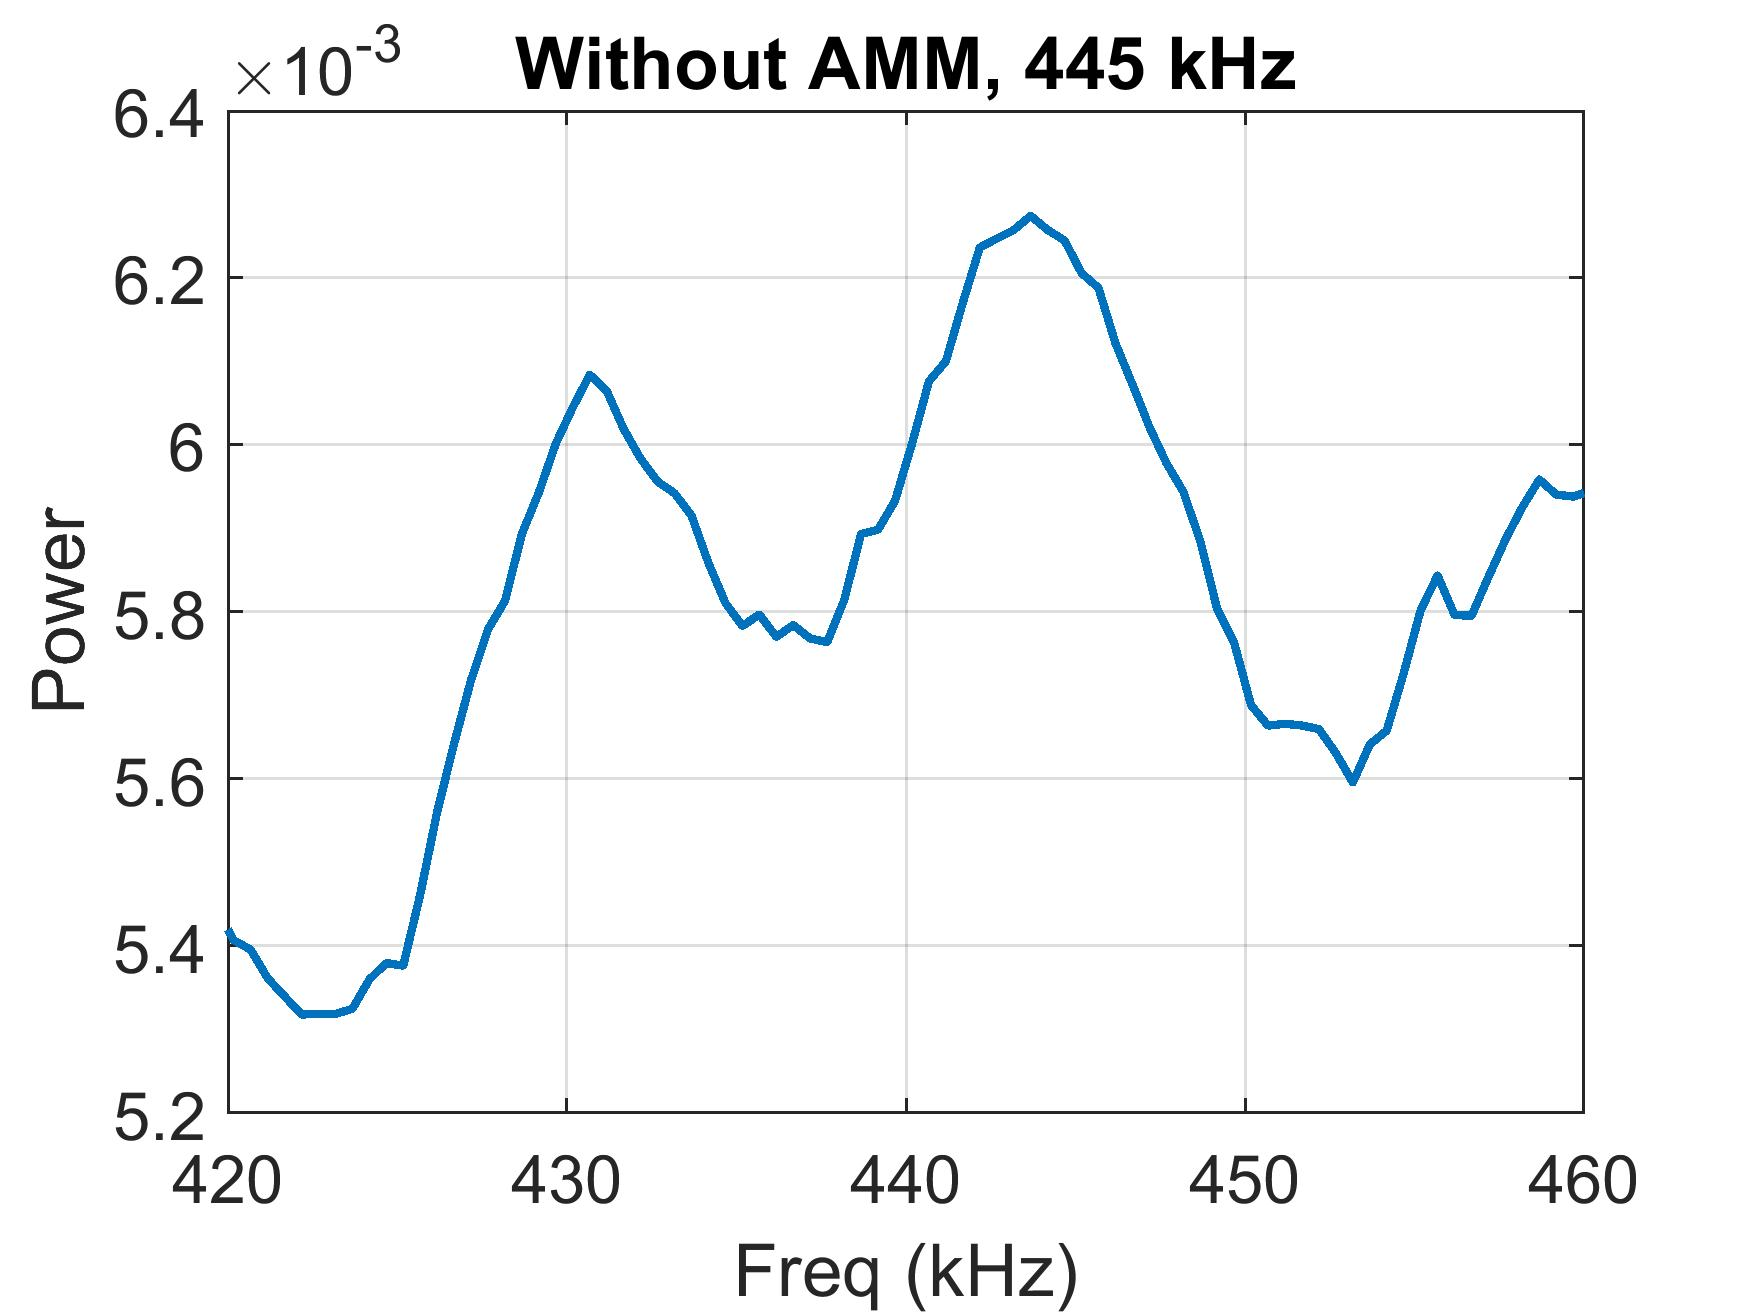
\includegraphics[width = \textwidth]{../../matlab/exp/fig/CalPowTransCoef_230302C_PowVoid.jpg}
    \end{subfigure}
    \begin{subfigure}{0.32\textwidth}
        \centering
        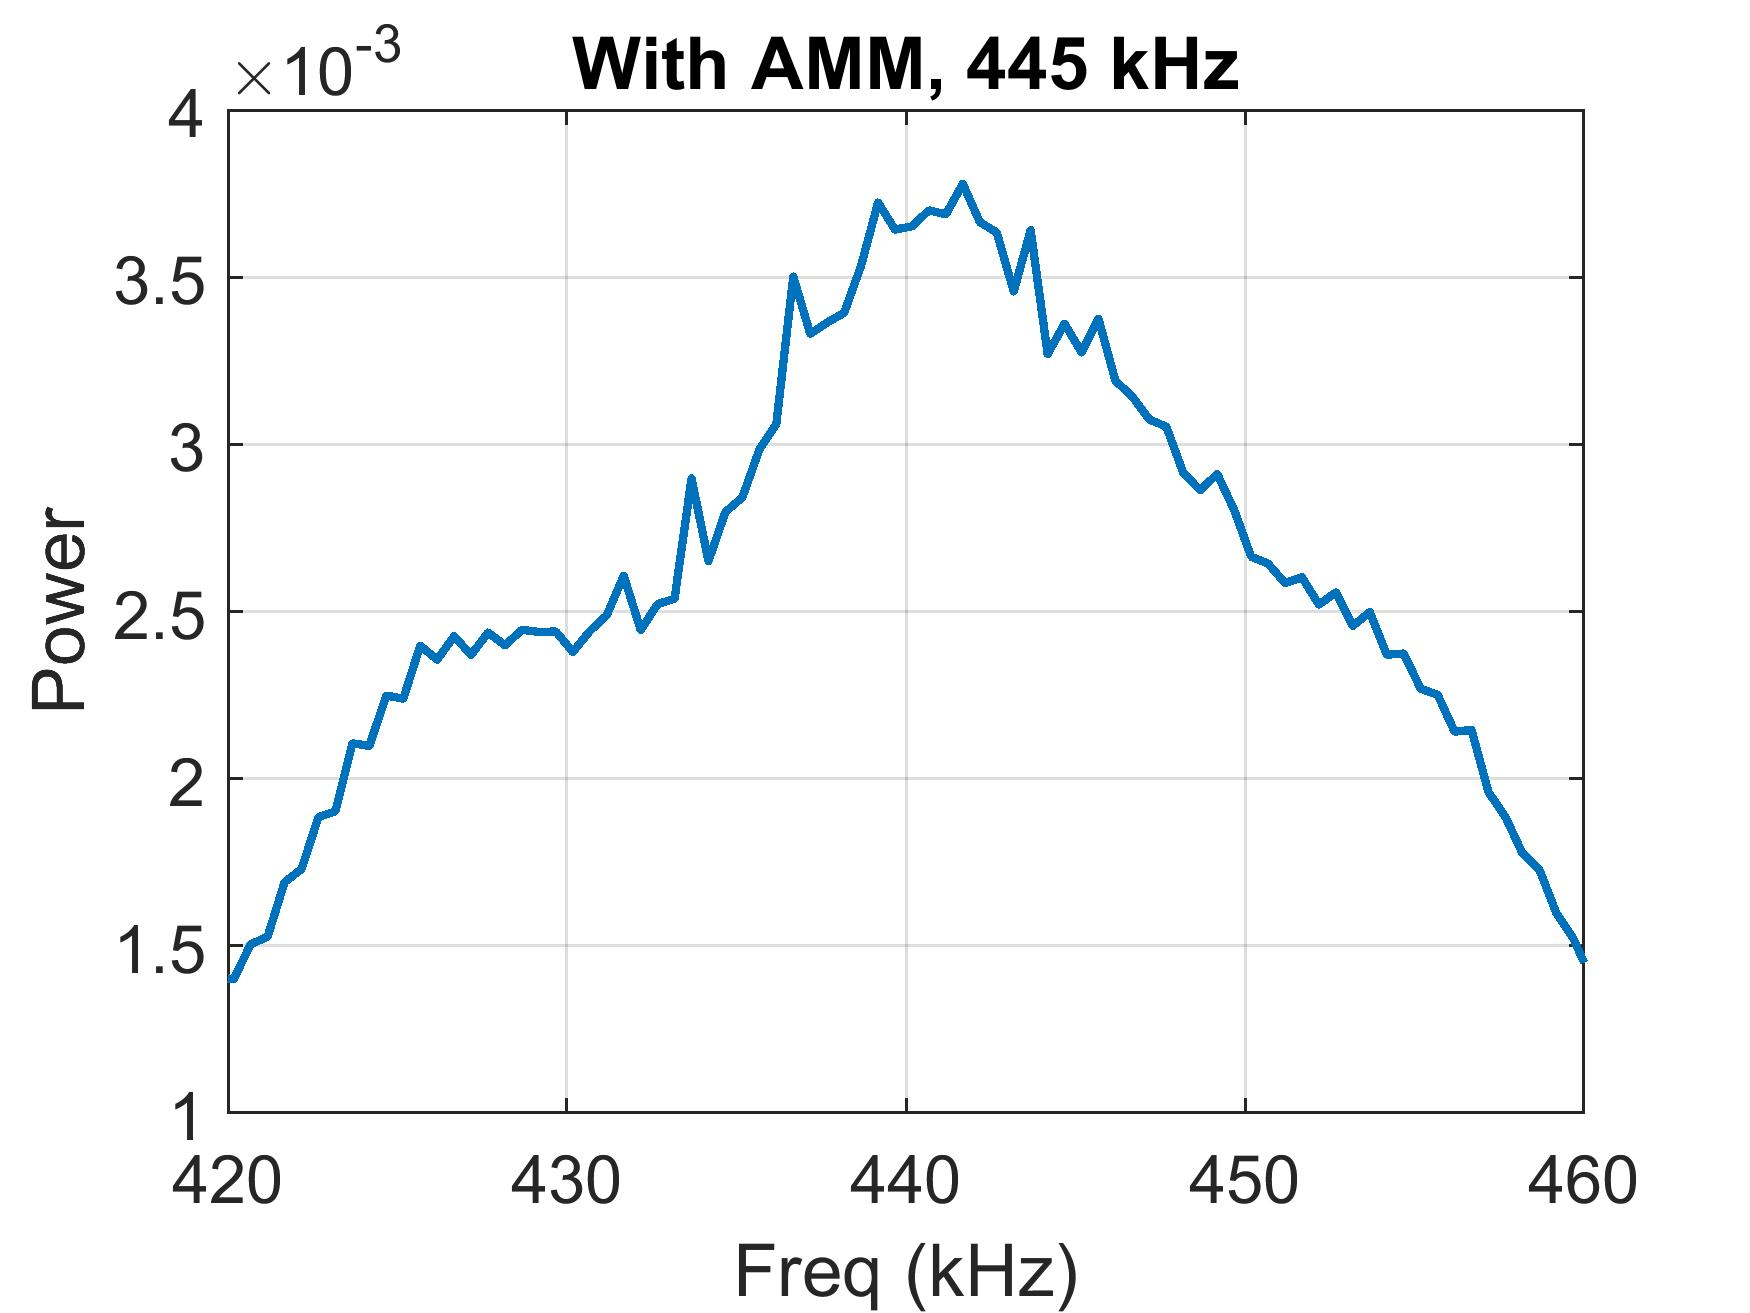
\includegraphics[width = \textwidth]{../../matlab/exp/fig/CalPowTransCoef_230302C_PowAMM.jpg}
    \end{subfigure}
    \begin{subfigure}{0.32\textwidth}
        \centering
        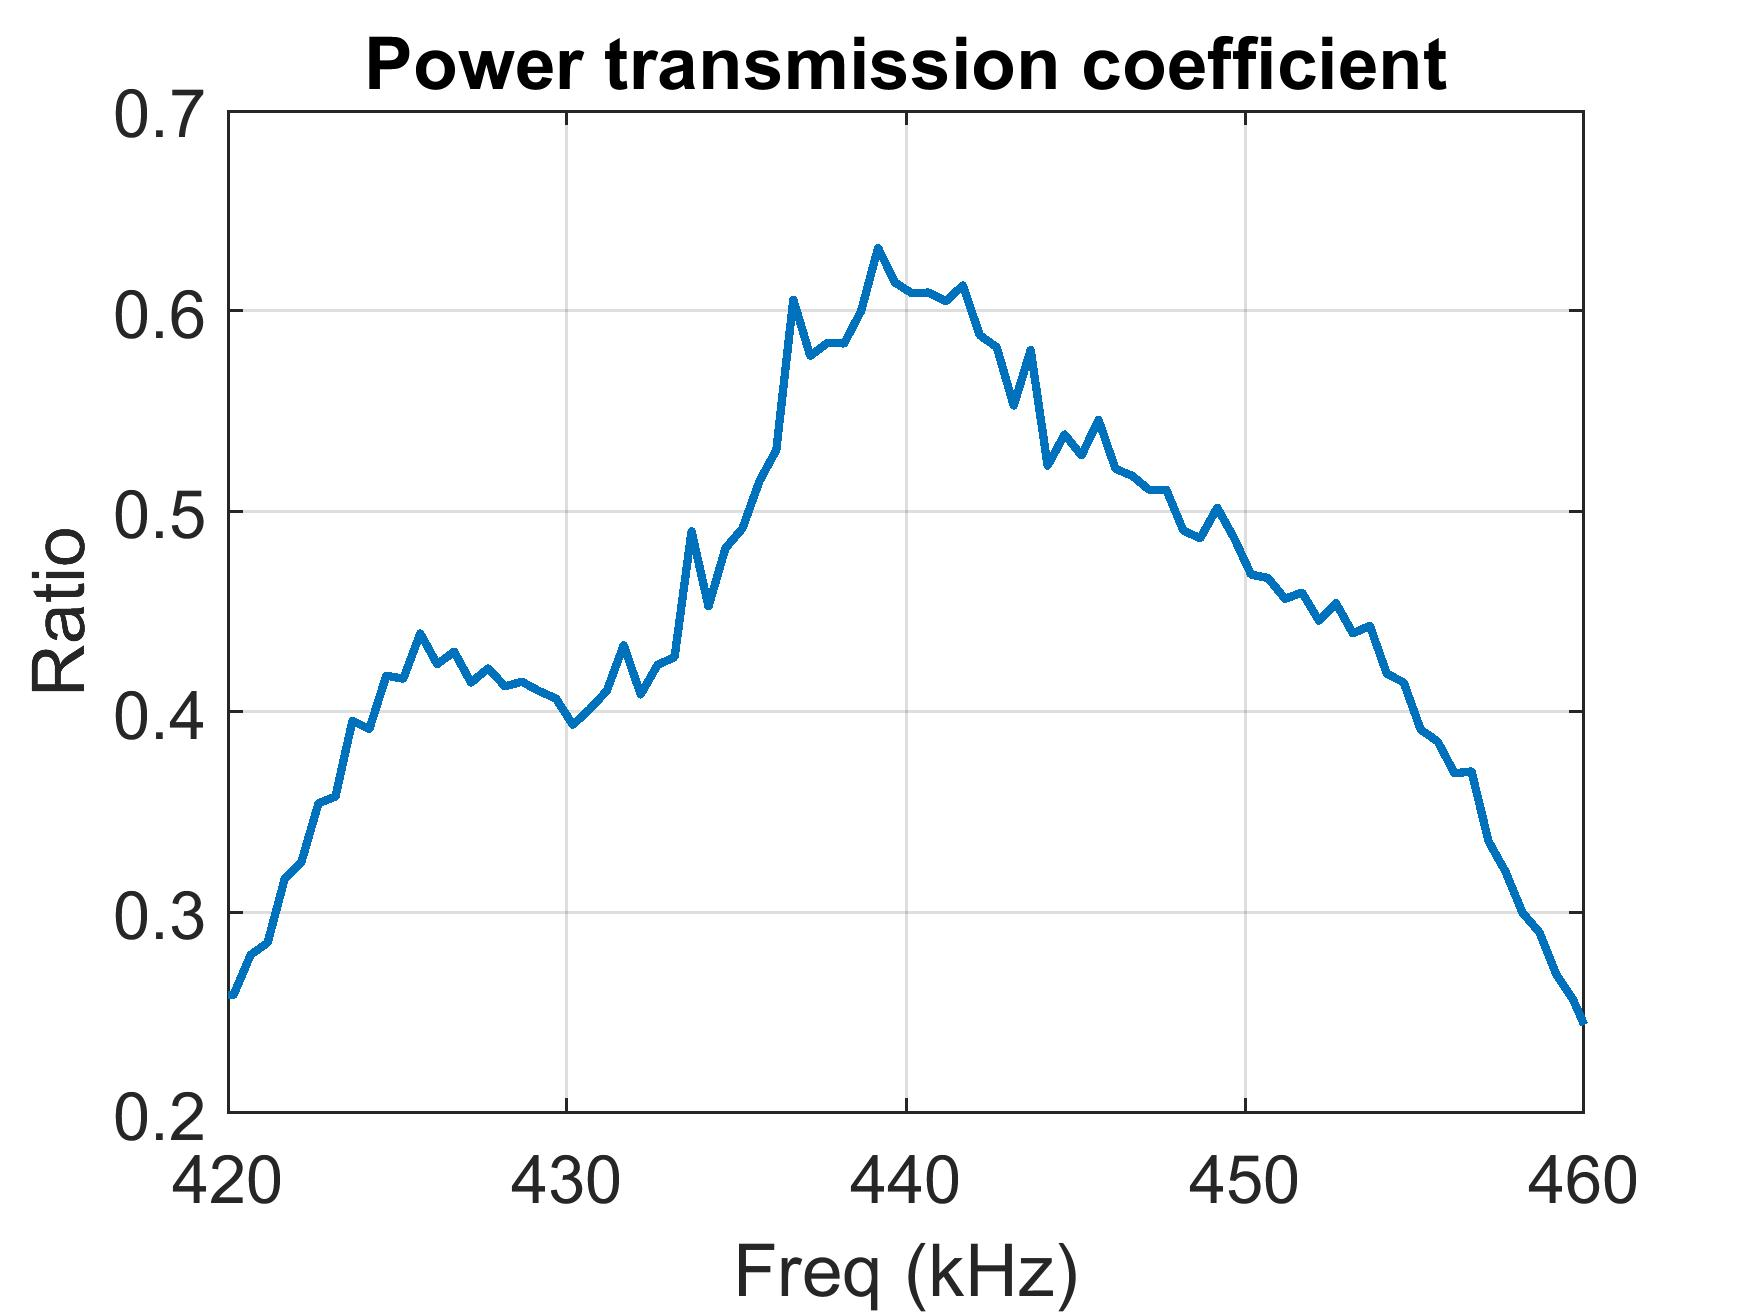
\includegraphics[width = \textwidth]{../../matlab/exp/fig/CalPowTransCoef_230302C_PowCoefAMM.jpg}
    \end{subfigure}
    \caption{
        Sound power (left) without and (middle) with the AMM.
        (Right) Power transmission coefficient.
    The region is located at 45~mm away from the transducer.}
    \label{fig:f9j:0213921j09j}
\end{figure}




% Activate the appendix
% from now on sections are numerated with capital letters
\begin{appendices}
% \addcontentsline{toc}{section}{Appendices}

\section{TBD}

\end{appendices}


\addcontentsline{toc}{section}{References}
\bibliographystyle{unsrt}
\bibliography{zotero}

\end{document}



